\documentclass{article}
\usepackage{graphicx} % Required for inserting images
\usepackage{placeins}
\usepackage{venndiagram}
\usepackage{tikz}

\title{Exploring Bayesian Statistics: A Review of 'Bayesian Statistics The Fun Way'}
\author{Shibo Liu}
\date{November 6th 2023}

\begin{document}

\maketitle

\section{Introduction}
The Bayesian Statistics has captivated my intellectual curiosity for an extended duration. Nowadays, Bayesian Statistics plays an increasingly critical role, extending beyond its traditional domain in Statistics and infiltrating cutting-edge technologies like artificial intelligence, particularly within the field of machine learning. As a graduate student in electrical and computer engineering, my statistical knowledge has predominantly revolved around frequentist methods. However, this project presents an invaluable opportunity for me to explore the Bayesian Statistics. In this paper, I will expound upon various crucial concepts in Bayesian statistics, as elucidated in the book 'Bayesian Statistics The Fun Way,' and explore their potential applications.

\section{Revisit Bayes' Theorem}
The Bayes' Theorem can be derived from conditional probability, which refers to the probability of event A occurring when event B occurs, represented by $P(A|B)$.
\begin{figure}[!htbp]
    \centering
    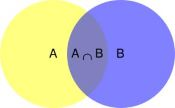
\includegraphics{Picture2.jpg}
    \caption{Venn diagram of the intersection of two events}
    \label{fig:enter-label}
\end{figure}
\FloatBarrier
According to the Venn diagram, it can be clearly seen that when event B occurs, the probability of event A occurring is:
\[P(A|B)=\frac{P(A \cap B)}{P(B)}\]
Rearrange the equation,
\[P(A \cap B)=P(A|B)P(B)\]
Similarly,
\[P(A \cap B)=P(B|A)P(A)\]
Therefore, we could get the mathematical representation of Bayes' Theorem:
\[P(A|B)=\frac{P(A)P(B|A)}{P(B)}\]
This representation of Bayes' Theorem might not be immediately intuitive upon first glance. To better understand it, I would further explain it by highlighting the relationship between our observation and belief:\\\\
Let B denote belief and O denote observation.
\[P(B|O)=\frac{P(B)P(O|B)}{P(O)}\]
This formula can be split into four parts:
\begin{enumerate}
    \item $P(O|B)$: This component is commonly referred to as the likelihood function. It quantifies the probability of observing data (O) given our initial beliefs (B). Essentially, it measures how likely the observed event is based on our pre-existing understanding of the world.
    \item $P(B)$: This term is typically known as the prior function, representing our initial beliefs before taking any observations into account.
    \item $P(B|O)$: Commonly called the posterior function, it signifies the updated probability of our beliefs (B) after incorporating new evidence or observations (O). In essence, it reflects how our initial beliefs should be revised in light of the observed data.
    \item $P(O)$: This component signifies the total probability of observing a specific set of data, without regard to our initial beliefs or hypotheses. Within the framework of Bayes' theorem, it serves as a normalization factor, ensuring that the updated probability constitutes a valid probability distribution.
\end{enumerate}
One of the most captivating aspects of Bayes' Theorem lies in its unique capacity to merge our initial beliefs about the world with the empirical data we collect, resulting in an updated assessment of the reliability of our beliefs in light of the evidence at hand. This feature distinguishes Bayes' Theorem from traditional statistics, as traditional methods lack the ability to incorporate prior knowledge into their analyses.\\\\
In traditional statistics, the analysis primarily relies on observed data and typically excludes the explicit inclusion of prior beliefs or subjective information. However, when we leverage Bayes' Theorem in conjunction with our existing beliefs and observations, we empower ourselves to adapt our initial convictions and permit evidence to influence the strength of our beliefs.\\\\
Our initial beliefs are usually our starting level of confidence in an idea, represented as \(P(A)\) in Bayes' Theorem. Frequently, we engage in debates on subjects such as the climate change policies. But we may not always consider how new evidence should alter our perspectives or those of the individuals we are debating with.\\\\
Bayes' Theorem provides a framework for us to appraise the evidence related to these beliefs and to quantify precisely how this evidence should modify our beliefs. This ability to update our beliefs in response to evidence is a cornerstone of Bayesian thinking, making it a powerful tool in fields like machine learning, medical diagnosis and so on.
\section{Apply Bayes' Theorem to Hypothesis Testing and Parameter Estimation}
\subsection{Hypothesis Testing}
The hypothesis testing is a fundamental component of statistical analysis. It begins by formulating two hypotheses: the null hypothesis and the alternative hypothesis. Data is collected, and a significance level is chosen to determine the threshold for statistical significance. A test statistic is then calculated based on the data and the null hypothesis, with the choice of test statistic depending on the specific test being conducted. The critical region, derived from the significance level and the test statistic's probability distribution, is defined to decide when to reject the null hypothesis. Comparing the test statistic to critical values, the null hypothesis is either rejected or not. The results are reported, including the test statistic's value and the decision made, often aided by the p-value, which quantifies the evidence against the null hypothesis. This traditional approach provides a systematic methodology for evaluating hypotheses and drawing conclusions based on observed data but has obvious limitations. It typically focuses on either accepting or rejecting the null hypothesis based on p-values and preset significance levels, which can be somewhat rigid and lead to black-and-white conclusions. Furthermore, the null hypothesis and alternative hypothesis must match with each other, which means we could not have two equations for each. Additionally, it lacks the capacity to directly incorporate prior knowledge.\\\\
Bayesian hypothesis testing offers a novel and powerful alternative to traditional frequentist hypothesis testing methods, addressing some of their inherent limitations.  Bayesian hypothesis testing, on the other hand, allows for a more flexible approach. Instead of merely accepting or rejecting hypotheses, it provides a framework for quantifying the degree of belief or uncertainty in various hypotheses by incorporating prior knowledge and updating it with new data. This approach provides a richer and more informative way to evaluate hypotheses, making it particularly useful when dealing with complex scientific questions and cases with limited data. Bayesian hypothesis testing offers a more comprehensive and intuitive way to assess hypotheses while accounting for the inherent uncertainty in real-world scenarios. Here, I will explain how Bayes' Theorem works in the context of hypothesis testing.
\subsubsection{Prior Odds}
The prior odds are defined as the ratio of prior probabilities:
\[O(H_1)=\frac{P(H_1)}{P(H_2)}\]
This ratio compares the probability of two hypotheses before we look at the data. This representation is helpful because it lets us easily note how strongly we believe in the hypothesis we are testing without any other information. When this number is greater than 1, it means the prior odds favor our hypothesis and when it is a fraction less than 1, it means they are against our hypothesis. For instance, if we have $O(H_1)=100$, it indicates that, in the absence of any further data, we believe that the probability of $H_1$ is 100 times greater than that of the alternative hypothesis.
\subsubsection{Bayes Factor}
The Bayes Factor is defined as the ratio between the likelihoods of two hypotheses:
\[\frac{P(D|H_1)}{P(D|H_2)}\]
This concept holds a special place in Bayesian Statistics because it shifts the focus from gathering evidence to validate our ideas to a more profound exploration of how well our ideas elucidate the observed evidence. This ratio serves as a metric for assessing the plausibility of our observations within the context of our beliefs and someone else's beliefs. Our hypothesis wins when it explains the world better than the competing hypothesis. If the competing hypothesis explains the data much better than ours, it might be time to reassessment our beliefs. In Bayesian Statistics, the primary concern isn't supporting our beliefs; rather, it revolves around evaluating the degree to which our beliefs align with the data we encounter. Ultimately, data can either substantiate our ideas or prompt a reconsideration of our standpoint.
\subsubsection{Posterior Odds}
By putting the prior odds and bayes factor together, we could get the posterior odds:
\[posterior\ odds=O(H_1)\frac{P(D|H_1)}{P(D|H_2)}\]
The posterior odds calculates how many times better our hypothesis explains the data than a competing hypothesis. In the book it gives a guideline for interpreting the result of posterior odds.
\begin{table}[!htbp]
    \centering
    \begin{tabular}{cc}
        Posterior Odds & Strength of evidence\\
        1 to 3 & Interesting but nothing conclusive\\
        3 to 20 & Looks like we're on something\\
        20 to 150 & Strong evidence in favor of $H_1$\\
        $>150$ & Overwhelming evidence\\
    \end{tabular}
    \caption{Guidelines for evaluating posterior odds}
    \label{tab:my_label}
\end{table}
\FloatBarrier
While these values can be helpful as a general reference, I believe that case-by-case evaluation is still necessary. For instance, if we're in a friendly debate with someone and our posterior odds are 2, it might be enough to make us feel quite confident. However, when it comes to determining if something we're about to eat is safe or poisonous, a posterior odds of 100 might still not be sufficient to ensure our safety.\\\\
The book has outlined the advantages of Bayesian Statistics compared to the traditional approach. However, the question arises: why is the traditional approach still so prevalent today? I will now give my answer and provide an example to illustrate this point.\\\\
Let's consider an example: Suppose both you and your friend are attempting to predict the outcome of a roll of a six-sided die. You argue that the probability of guessing correctly is $\frac{1}{6}$, while your friend, drawing from their past experiences, suggests a probability of $\frac{9}{10}$. Now we have two hypotheses:
\[H_1:P(correct)=\frac{1}{6}\]
\[H_2:P(correct)=\frac{9}{10}\]
Now we calculate the Bayes Factor:
\[Bayes\ Factor = \frac{P(D_{10}|H_2)}{P(D_{10}|H_1)}=\frac{(\frac{9}{10})^9\times (1-\frac{9}{10})}{(\frac{1}{6})^9\times (1-\frac{1}{6})}=468517\]
The likelihood ratio indicates that $H_2$ provides an explanation for the data that is 468,517 times more favorable than $H_1$. This finding raises some concerns for you, but it hasn't yet been integrated with the prior odds.\\
Considering that, in common sense, correctly guessing the outcome of a six-sided die 9 out of 10 times is extremely challenging, it seems reasonable to establish the prior odds strongly in favor of $H_1$ to cancel out the Bayes Factor.
\[O(H_2)=\frac{1}{468517}\]
Now when we calculate the posterior odds we find that both hypothesis are at the same stage again:
\[posterior=O(H_2)\times\frac{P(D_{10}|H_2)}{P(D_{10}|H_1)}=1\]
But suppose your friend rolls the die five more times and successfully predicts all of them. Now the observations are updated and if we look at the posterior now:
\[posterior'=O(H_2)\times \frac{P(D_{15}|H_2)}{P(D_{15}|H_1)}=\frac{1}{468517}\times \frac{(\frac{9}{10})^{14}\times (1-\frac{9}{10})}{(\frac{1}{6})^{14}\times (1-\frac{1}{6})}=4592\]
Using the existing prior with just five more rolls of die, the posterior becomes 4592 now, which means we are strongly certain that $H_2$ is correct. 
\\\\
In the provided example, the challenges associated with Bayesian statistics in hypothesis testing become apparent. The key factors explaining this situation include the subjectivity of prior probabilities and the need to specify them. Bayesian statistics require prior probabilities, which can be highly subjective and vary among individuals, potentially leading to disagreements in their selection. This subjectivity introduces bias and reduces objectivity in the analysis. Furthermore, in the example, even a slight adjustment in the prior odds had a significant impact on the posterior odds, emphasizing the influence of prior beliefs. This makes it crucial to carefully set the prior probabilities, but it also highlights their subjectivity, which can be challenging to navigate in practice.
\subsection{Extend Hypothesis Testing to Parameter Estimation}
It is notable that Bayesian Statistics offers a clear advantage: it allows for the inclusion of multiple equations for alternative hypotheses. This flexibility enables us to explore a virtually continuous range of potential hypotheses. Consequently, the posterior odds, traditionally used for hypothesis testing, can also serve as a means for parameter estimation. This process is typically facilitated through programming, which involves searching for the posterior odds for every conceivable hypothesis. The figure below provides an illustration of this process.
\begin{figure}[!htbp]
    \centering
    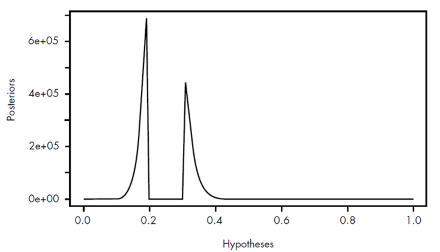
\includegraphics{Picture3.png}
    \caption{Posterior as a function of Hypothese}
    \label{fig:enter-label}
\end{figure}
\FloatBarrier
As evident from the figure above, the parameter estimation is likely around $p=0.2$. However, as previously emphasized in hypothesis testing, it's crucial to interpret these results within the context of a specific scenario. Sometimes the hypothese with the biggest posterior may not necessarily provide the optimal parameter estimation.
\end{document}
